\RequirePackage[l2tabu, orthodox]{nag}
\documentclass{report}

\usepackage[T1]{fontenc}
\usepackage{microtype}
\usepackage{lmodern}
\usepackage{microtype}
\usepackage{comment}
\usepackage{mathtools}
\usepackage{dsfont}
\usepackage{amssymb}
\usepackage{bbm}
\usepackage{algorithm}
\usepackage[noend]{algpseudocode}
\usepackage[dottedtoc]{classicthesis}
\usepackage{amsthm}
\usepackage{diffcoeff}
\usepackage{cleveref}
\usepackage{subcaption}
\usepackage[]{graphicx}
\usepackage{tikz}
\usepackage{tikz-cd}
\usepackage{float}
\usepackage{lipsum}
\usepackage{siunitx}
\usepackage[colorinlistoftodos]{todonotes}
\usepackage[sorting=none]{biblatex}
\usepackage{url}
\usepackage{neuralnetwork}
\usepackage{afterpage}

\newcommand\blankpage{%
    \null
    \thispagestyle{empty}%
    \addtocounter{page}{-1}%
    \newpage}

\usetikzlibrary{positioning,chains}

\DeclarePairedDelimiter\abs{\lvert}{\rvert}%
\DeclarePairedDelimiter\norm{\lVert}{\rVert}%


\addbibresource{references.bib}

\title{Monte-Carlo Regularization}
\author{Jakob Huber}
\date{\today}

\begin{document}
    \begin{titlepage}
    
    ~\\
    \makebox[0pt][l]{%
    \begin{minipage}[b]{0.25\textwidth}
    ~\\
    \end{minipage}
    \begin{minipage}{0.65\textwidth}
    \begin{flushleft}
    \vspace{4cm}
    {\fontsize{28}{24}\textbf{\sffamily Monte Carlo Regularization}\\}
    \vspace{1cm}
    {\fontsize{19}{17}\sffamily by\\}
    \vspace{1cm} 
    {\fontsize{16}{18}\textbf{\sffamily Jakob Huber}}\\
    \end{flushleft}
    \end{minipage}
    }

    \vspace*{\fill}

    \begin{flushleft}
    \noindent
    Degree Project in Theoretical Physics (30 ECTS credits)\\
    Master's Programme in Engineering Physics\\
    KTH \textit{Royal Institute of Technology, 2020}\\
    Supervisor at KTH: Prof. Egor Babaev\\
    Examiner at KTH: Jack Lidmar\\
    Supervisor at Rumbline Consulting AB: Dr. Siril Yella
    \end{flushleft}
    
\end{titlepage}
    
    \pagenumbering{roman}

    \newpage
\thispagestyle{plain}
~\\
\vfill
{ 
	\subsection*{Authors}
	Jakob Huber <jhuber@kth.se>\\
	School of Engineering Sciences\\
	KTH, \textit{Royal Institute of Technology}
	
	\subsection*{Place for Project}
	\textbf{KTH} SCI\\
	SE-100 44 Stockholm, Sweden

	\subsection*{Examiner}
	Jack Lidmar <jlidmar@kth.se>\\
	Department for Theoretical Physics \\
	KTH, \textit{Royal Institute of Technology}
	
	\subsection*{Supervisor KTH}
	Prof. Egor Babaev <babaev@kth.se>\\
	Department for Theoretical Physics\\
	KTH, \textit{Royal Institute of Technology}


	\subsection*{Supervisor Company}
	Dr. Siril Yella \\
	Rumbline Consulting AB
}


\newpage
\thispagestyle{plain}
%%%%%%%%%%%%%%%%%%%%%%%%%%%%%%%%%%%%
%%  The English abstract          %%
%%%%%%%%%%%%%%%%%%%%%%%%%%%%%%%%%%%%
\chapter*{Abstract}
%%%%%%%%%%%%%%%%%%%%%%%%%%%%%%%%%%%%

Statistical models bear the inherent problem of overfitting, consisting of more parameters than justifiable based on the data. For artificial neural networks, computing abstractions of biological neural networks, the parameters consist of artificial neurons and connections. The challenge of overfitting is explored by introducing a regularization scheme by a dynamical structural evolution for an artificial neural network in training. A novel statistical physics-inspired algorithm is proposed by inserting or deleting parameters by cross-validation on a selection data set. The regularization consists of generating perturbations of the neural net structure and randomly adopting among the most positive alterations. These operations are formalized to allow for generalization and application on any neural net set-up. A proof-of-concept is sought for the algorithm with a fully connected recurrent neural network and tested on a supervised learning task using the MNIST data set. The algorithm is shown to benefit small to medium-sized networks on the tested data set and diminishes the hidden layer size's overall effect on test set performance. With proper scaling, the proposed algorithm could benefit artificial neural networks with arbitrary structure and size.


\subsection*{Keywords}
regularization, machine learning, AI, statistical physics, neural networks, deep learning


\newpage
\thispagestyle{plain}
%%%%%%%%%%%%%%%%%%%%%%%%%%%%%%%%%%%%
%%	 The Swedish abstract         %%
%%%%%%%%%%%%%%%%%%%%%%%%%%%%%%%%%%%%
\chapter*{Abstract}
%%%%%%%%%%%%%%%%%%%%%%%%%%%%%%%%%%%%
Statistiska modeller har det inneboende problemet med överanpassning, de kan bestå av fler parametrar än motiverat baserat på data. För artificiella neurala nätverk, datorabstraktioner av biologiska neurala nätverk, består parametrarna av artificiella nervceller och anslutningar. Utmaningen med överanpassning utforskas genom att införa ett system för regularisering genom en dynamisk strukturell utveckling för ett artificiellt neuralt nätverk under träning. En ny statistisk fysikinspirerad algoritm föreslås genom att infoga eller ta bort parametrar genom korsvalidering på en urvalsdatauppsättning. Regulariseringen består i att generera störningar i den neurala nätstrukturen och slumpmässigt anta en bland de mest positiva förändringarna. Dessa operationer är formaliserade för att möjliggöra generalisering och tillämpning på alla neurala nätuppsättningar. Ett bevis på koncept eftersträvas för algoritmen på ett fullt anslutet återkommande neuralt nätverk och testas på en övervakad inlärningsuppgift på MNIST-datauppsättningen. Algoritmen har visat sig gynna små till medelstora nätverk på den testade datamängden och minskar det dolda lagrets storleks totala effekt på testuppsättningens prestanda. Med korrekt skalning kan den föreslagna algoritmen gynna artificiella neurala nätverk med godtycklig struktur och storlek.

\subsection*{Nyckelord}
regularisering, maskininlärning, AI, statistisk fysik, neurala nätverk, djup maskininlärning


\newpage
\thispagestyle{plain}
\chapter*{Acknowledgements}
I want to express thanks to my supervisor Prof. Egor Babaev at KTH, for providing the problem of this thesis and supervision. Dr. Siril Yella at Rumbline Consulting for structure and feedback on my report. Per Ininbergs at Rumbline Consulting for support and motivation in what comes after the thesis. Wile Balkhed and Viktor Nilsson for reminding of the importance of general time management and thesis writing. 

I would most like to thank my supervisor Emil Blomquist at KTH for supervising and collaborating. Also, giving me this opportunity and the hard work put into start-off and exploring in a new direction.

\newpage

\thispagestyle{plain}

\tableofcontents

\newpage
\pagenumbering{arabic}



    
\chapter{Introduction}

In this master thesis, the prospect of a recurrent neural network, RNN, with a stochastic structure varying in time to regularize it, Monte Carlo regularization, MCR, is presented. A regularization technique is introduced to combat overfitting for the neural network. Inspiration is drawn from biology, where neural networks organically evolve their structure, formalized in the concept of a Markov process. However, how this algorithm is structured is inspired by the physics processes of grand-canonical ensembles or processes where energy differences drive the algorithm — evaluating the energy differences of either pruning or duplication of neurons, thus regulating the structure of the neural net.

\section{Recurrent Neural Network - History}

RNNs are a class derived from feed-forward neural networks with iteration over a fixed structure to achieve temporal dynamics \cite{DRNNS}. Forming along the time axis is a directed graph, achieving dynamic behavior in the sense of memory. Utilizing the memory to capture patterns also requires dynamical programming for the necessity of mapping long sequences to short or vice versa. The RNNs excel at pattern recognition in data sequences, e.g., natural language processing, machine translation, and most commonly speech recognition \cite{handwriting}. Their recurrent structure could strain this process of regularization and are therefore tested on.

Initially, RNNs were called dynamic recurrent neural networks, DRNs, displaying time-varying responses as per dynamical systems. During the early stages of development, a vital issue was shown by Bengio \cite{ben}, that the necessary condition for the system to robustly store discrete state information for the long-term results in a sufficient condition of gradient decay. The issue of vanishing gradient \cite{hoch} or exploding thereof when training RNNs, affecting long-range temporal dependencies, hinders the ideal application. 

Launching RNNs has thus been slowed as despite the straightforward concept introduced in 1986 \cite{RNN1}, implementing has been fraught with difficulties in capturing long-range temporal dependencies and slow computation. With advances in hardware, these problems have been somewhat mitigated, and RNNs exist in modern applications. However, the prospect of keeping RNNs small or NNs, in general, is engaging.

The vanishing gradient phenomenon can be exemplified when utilizing the conventional training algorithm backpropagation through time, BPTT, first unfolding the network, then backpropagating the error through the network \cite{DRNNS}. Small changes permeate the network, possibly causing exponential diminishing or increase of individual later weights in the network, affecting the gradient \cite{field}. Additionally, with this naïve algorithm, unfolding and effectively producing a feed-forward network, training would be impossible for a large number of iterations. An attempt at solving this is by truncating and not unfolding the whole network at every step, possibly using parallelization to calculate in parts. However, this would consequentially truncate long-term dependencies simultaneously. Seemingly a Mexican stalemate, efforts to remedy this have been somewhat successful. 

One early method of mitigating the effects came with so-called NARX networks (Nonlinear AutoRegressive with eXogenous inputs method) \cite{DRNNS}, which introduce direct connections between current and past hidden states, reducing nonlinearities inherent in the RNN structure. However, these architectures only alleviate by a constant factor the duration of temporal dependencies that can be learned \cite{suts}.

A stochastic approach termed the echo state network, ESN, employs random connections but suffers from sizeable structural overhead and is unable to cope with data-intensive problems. The method stems from the more general approach of random weight guessing, RG, which suffers in complex structures only being reliable under solution-dense conditions. RG could be used in benchmark evaluation for identifying faulty design. Moreover, the random structure's impressive performance in specific domains suggests that it is worth investigating ESN-based initialization \cite{suts} or expanded random features. 

Leading RNN architecture is the long short-term memory \cite{LSTM}, LSTM, which is currently in use in state-of-the-art speech recognition and smart assistants \cite{Apple}. The LSTM uses memory units, linear and adept at controlling information to and from the unit, productively truncating the gradient without undermining performance. There has been further development and improvement on the LSTM structure, and several variants have been devised, tests have been conducted, and overall comparable performance was confirmed\cite{Greff}. The Gated recurrent units, GRUs, akin to the LSTM but with fewer parameters, are commonly applied alterations but has been shown to be lesser than the LSTM in application. However, complex models require more training. As has been established, LSTM has proceeded to solve pathological long-range temporal dependencies and was successfully applied to speech and handwritten text recognition \cite{gs, gas}, robotic control \cite{mayer}. Attempts have been made to progress further, putting LSTMs in a grid\cite{ka} or, in combination with generative models and evaluation seems promising\cite{gr, ch, bo}. In conclusion, RNN and especially LSTM belong to the principally most general and powerful sequence processors out there.

LSTM has clear advantages over conventional RNNs; however, with the coming of Hessian free optimization, HF, in addition to structural dampening, this edge is lessened. With the method, RNNs proceed to solve pathological long-term dependencies, computationally it still lacks in comparison \cite{suts}. 

From the RNN formulation above, a problem with RNNs is the mapping of long to short sequences, which has been recently treated with attention-based models \cite{xu}. Earlier, the solution consisted of compressing the input, meanwhile losing information and spending resources compressing. Attention-based models brought the implementation of variable length memory, which gives flexibility in generating the output and accessing different parts of the memory at different output times. 

The active field of capturing long-time dependencies has been a focus, especially for RNNs and in different ways avoiding the structure altogether seems to be the most recent advancements. However, the application of an in part pruning algorithm on an RNN is of interest as this could point to the versatility and benefit of such algorithms.

Besides the ones mentioned, challenges ahead include faster learning, representational capacity, and weights as states \cite{suts}. Faster learning relates to the high cost of calculating the gradient on long sequences; methods to approximate derivatives under such circumstances quickly and efficiently are crucial. The two latter pertain to the hidden state's size, the information, and computation related to a sequence; by increasing the size, it is possible to achieve longer-term temporal dependencies. The hidden state's size is where the proposed algorithm's stochastic nature, changing the structure through time, aims to increase the hidden state's size.

\section{Regularization}

Apart from these challenges, for RNNs, a more general problem for any statistical model is overfitting. This phenomenon spawns when an NN model includes more adjustable parameters than necessary, or an overly complicated way of achieving fitness is used. Specifically, overfitting violates Occam's razor in which any given complex function is a priori less probable than any given simple function. Battling overfitting regularization schemes are introduced. Overfitting is increasingly likely to happen by prolonging the training scheme, and the necessity for regularization increases.

Several forms of regularization exist. A term is commonly added to the optimization problem, which penalizes the sought function's complexity. A typical example is the Tikhonov regularization, which adds the L2-norm of the supposed solution and thus preferring smaller norms. The motivation for regularization is improving the generalization of the learned model; in this case, smaller norms equal better generalization. Other regularization examples include early stopping, which incorporates a statistically independent validation set on which performance is measured, and training continues until performance no longer improves. Pruning is another method in which one targets connections or parameters of the NN itself and removing them, producing sparse networks but this entails retraining the pruned network \cite{Yann}. The removal is decided by calculating either the sensitivity of removing weights on the cost function or only the magnitude of each weight, claiming that relatively small magnitudes have small effects on the cost function. Additionally, a validation set can be used to cross-validate the cost function improvement on a separate set \cite{prunings}. 

The introduced algorithm is a regularization scheme that varies the structure to improve performance and simultaneously reduce the NN complexity. Firstly moves or changes are defined to limit how a NN can be changed. Starting from a fully connected network and changing the structure throughout the training. The proposed moves are deleting a node, duplicating a node, and deleting a weight or edge. The NN is first trained on the part of the data set, called the training set. The NNs structure is then perturbed in the moves described above, measuring energy before and after each separate move is made. The moves are benchmarked on an external data set, distinct from the training set called selection or validation set, to promote generalization. Based on the energy differences in the cost function of each of said moves, a softmax decision scheme is used to determine the move made. 

The thesis will consider a proof-of-concept of the introduced algorithm and regularization, using HF optimization for the RNN. Additionally, the algorithm will treat the standard data set MNIST, Modified National Institute of Standards and Technology\cite{mnist}. A possible novel application is the regularization of other neural networks when prompted by the suggested method.%here

Within deep learning, the other competing model is the convolutional neural network, CNN. This class is most commonly applied to image recognition or analyzing visual imagery in general. However, as of late, a variation has been designed to compete with RNNs on processing sequences, the so-called temporal CNN. Recent studies have been made showing the superiority of said architecture over RNNs\cite{tcnvsrnn}. However, the method presented is possibly applicable to CNNs too.

\section{Motivation}

Whenever a neural network, NN, is produced and benchmarked, there is a so-called "Brasklapp" that albeit the NN or NN-related algorithm performs well, there is a possibility that the hyperparameters regarding structure or other were not optimal. However, this is not a well-studied area. The implications of optimizing structure are a possible performance boost or faster training if a smaller NN could produce similar results. A pruning strategy is often implemented, effectively reducing the size and simultaneously the complexity of the NN.  

The task of hyperparameter optimization or restructuring is daunting and fraught with nonlinearities. In one way, it has been handled by generating a set of architectures, such as incrementally increasing the hidden layer and letting them go through the training procedure in parallel. This brute force method of testing some set of reasonable structures post-training completely avoids the problem and relies heavily on hardware; it is not a scalable method as the NN size increases, more computational power is required to in parallel train the NNs. The generated architectures are then benchmarked and cross-validated on a different set called selection set, which decides the then used NN. 

This thesis's effort is to streamline the procedure of perturbing architectures into an MC-walk; the randomness of the algorithm is introduced as there is no a priori optimal way to change the network. Regardless of the sophisticated method, in the end, what is strived for is a generalization. Firstly a set of moves or changes are decided. The moves are inspired by an organic NN where cells can divide or self-destruct, and their connections can change throughout the NN's lifetime. 

The induced changes are then thought of as fitness attributes, as in evolutionary biology, or a perturbance in which the most significant generated advantage should prevail. However, all data involved in the process only represent to a certain degree of the real test data set. Thus, selecting the best performing move is not guaranteed to generate, in the end, the best model. Ergo random factors decide which move to make; after more study, a preference could be established, such as always pruning the network. The duplication is included as even though the overall complexity might increase, on one level, redundancy is introduced and, as such, should not vastly change the intricacy. 

Similarly, the process could be thought of as a thermodynamic process proceeding towards equilibrium. Typically when simulating a grand-canonical ensemble, grand-canonical Monte Carlo is used. As is often the case, energy is minimized until only statistical fluctuations remain, treating changes in the NN of a mini-batch as such towards the end of the training. Additionally, particles, in this case, nodes or neurons, can be inserted or removed. The NN changes are sent through a similar scheme as in the simulation of the physical system; however, more consideration is taken when generating or deleting nodes as no governing distribution exists for NNs. This is due to the fact that distributions concerning NN parameters are problem adapted, akin to a configurational bias implementation of the Monte Carlo method. 

\section{Related Work}

The idea of modifying the structure of the neural network in time is not unfamiliar, and a related significant breakthrough is the dropout technique \cite{drop}. Both algorithms can be seen as adding noise to hidden units; the proposed stochastic structure, MCR, takes this one step further by allowing mutation. Formally a stochastic regularization technique, dropout attempts to increase generalization performance by reducing overfitting during learning. Similar to MCR, dropout instead tackles the challenge of overfitting by dropping units or nodes from the network, making the network simpler and thus easier to train. Additionally, this opens the possibility of combining exponentially many different network architectures efficiently, drawing from ensemble learning; this constitutes a pseudo-ensemble. However, dropout cannot be applied straightforwardly to RNNs \cite{dropno} but has to be limited to a certain subset\cite{droprnn} to be fruitful. The paper by \textcite{droprnn} only treats the LSTM structure and claim that it could be successfully applied to any RNN. 

Several other papers treat the issue by applying dropout to the connections in varying ways, limiting to the feed-forward network, only the non-recurrent connections or the hidden states update vector. Further modification includes the so-called Fracternal and Curriculum dropout or the stochastic depth; the last one consists of dropping an entire layer\cite{stochdep}. By combining the dropout method and DropConnect \cite{DropConnect}, a generalization of dropout for large fully-connected layers within structures and other methods resulted in a successful variant of the LSTM, namely the averaged stochastic gradient descent(ASGD) Weight-Dropped LSTM, AWD-LSTM for short. A landmark neural network architecture in language-modeling. 

Another approach is the so-called Zoneout\cite{zoneo}, where instead of dropout, a zoneout would revert the unit's activations to the previous timestep — injecting noise into the network, a mask designating which units are to be affected. Zoneout has the benefit of keeping propagation of gradients efficient and preserving state information, akin to feed-forward stochastic depth networks\footnote{Not to be confused with stochastic feed-forward neural networks. Despite their alluding name, stochastic feed-forward networks are related to Restricted Boltzmann Machines, RBMs, which learn probability distributions over its set of inputs.}. By optimally designating the occurrence of zoneout, state of the art advancements have been made\cite{Zoneout}. In the article by \textcite{Zoneout}, a concept surprise is introduced, the discrepancy between the last state's prediction and target. Surprisal could further be an optimum way of determining the stochastic evolution of MCR. The authors \textcite{Zoneout} conjecture that stochasticity leads to robustness in the hidden state. As mentioned, MCR is designed to increase the hidden state, and surprise implementation will be left out.

Weakening the stochastic activation of dropout in the sense of periodically managing information flow through the network is another method. One such model is the Phased LSTM \cite{phaselstm}, which specializes in asynchronous sensory events that carry timing information. Another is the Clockwork RNN \cite{Clockwork}, a NN architecture which partitions the hidden layer into distinct modules of temporal granularity, performing computations at its imposed clock rate. The proposed model takes one step into generalizing by delving into the stochastic forming of the network itself.

The attention-based model mentioned earlier was first introduced by \textcite{att}, improving the encoder decoder-based approach, which utilizes RNNs typically for machine translation. As RNNs and LSTMs still suffer from being unable to capture long data sequences, attention-based models are an effort to counter the problem by screening information. By weighing information based on a context given by the encoder, then generating a sentence from a picture or translating a sentence with the decoder, usually an LSTM. The concept has evolved into altogether attention-based architectures without RNNs such as the Transformer \cite{trans}, which has outperformed its predecessors. This introduced the notion of self-attention. The MCR could be thought of in a similar manner, where self-reflection is made to evaluate the current structure. 

Of general importance is the universal approximation theorem, which states that a feed-forward neural network is able to approximate any Borel measurable function on a compact domain. A proof has been done even for the case of RNN \cite{uarnn} and of interest is the particular evolving structure and its implications of the proposed MCR. However, this will not be studied in this thesis.

%attention, resnet, self-attention, tcm, hidden state theory, physics context
    
    \chapter{Model Description}

This section describes firstly the RNN structure and secondly the regularization.

\section{Differentiable Computational Graph}

Before introducing artificial neural networks as such, the mathematical foundation needs to be described as the regularization, to be well-defined, couples to the underlying theory of graphs. Most importantly is the efficient computation of derivatives of any function $F(\theta)$ that can be evaluated with such a graph. 

Considering a graph over $N$ nodes, $1, ..., N$ where $I$ is the subset consisting of the input nodes and $N$ is the output node. Each node $i$ has a set of ancestors $A_i$, determining its input, and a twice differentiable function $f_i$. For the above an algorithm for evaluating $F(\theta)$ on a computational graph:

\begin{algorithmic}[1]
    \State{Let $\theta$ be distributed between the input nodes $z_i, i \in I$}
    \For{$i=1$ to $N$ if $i\notin I$}
    \State{$x_i \gets \text{concat}_{j\in A_i}z_j$}
    \State{$z_i \gets f_i(x_i)$}
    \EndFor
    \Return{$F(\theta) = z_N$}
\end{algorithmic}

where every node $z_i$ can be vector valued.

Introducing a training error of the form $C(F(\theta)) = C(z_N)$, $C$ is the cost function and $F(\theta)$ is the models prediction on all samples. The derivative of $C(z_N)$ w.r.t. $\theta$ is given by $F'(\theta)^\top C'(z_N)$. The backpropagation algorithm calculates the product $F'(\theta)^\top v$ for arbitrary vector $v$ with according dimensionality $z_N$:

\begin{algorithmic}[1]
    \State{$dz_N \gets v$}
    \State{$dz_i \gets 0$ for $i<N$}
    \For{$i = N$ to $1$ if $i \notin I$}
    \State{$dx_i \gets f_i'(x_i)^\top dz_i$}
    \For{$j \in A_i $}
    \State{$dz_j \gets dz_j + \text{unconcat}^jdx_i$}
    \EndFor
    \EndFor
    \State{concatenate $dz_i$ for $i \in I$ onto $d\theta$}
    \Return{$d\theta = F'(\theta)^\top v$ }
\end{algorithmic}

\section{Recurrent Neural Network}

The recurrent neural network, RNN, is a nonlinear dynamical system mapping sequences to sequences. RNNs are typically structured with one input $i$, one hidden $h$ and one output layer $o$. Being parametrized by three weight matrices and two bias vectors \([W_{hi}, W_{hh}, W_{oh}, b_h, b_o]\) the state concatenation denoted \(\theta\) completely describes the RNN. Additionally an initial hidden state $h_0$ can be included but $h_0$ the initial hidden state is set to the zero vector in this thesis.

The forward propagation through the network of an input sequence \((i_1, i_2, ... , i_T)\) to an output sequence \((o_1, o_2, ..., o_T) \) is performed in the following algorithm:

\begin{algorithmic}[1]
    \For{$t$ from $1$ to $T$}
    \State{$u_t \gets W_{hi}i_t + W_{hh}h_{t-1} + b_h$}
    \State{$h_t \gets a_h(u_t)$}
    \State{$z_t \gets W_{oh}h_t + b_o $}
    \State{$o_t \gets a_o(z_t)$}
    \EndFor
\end{algorithmic}

where $h_0 = 0$. $a_h(*)$ and $a_o(*)$ are nonlinear activation functions for the hidden and output layer respectively. The cost function is usually defined as a sum of per-timestep cost:

\[C(o, y) = \sum_{t=1}^{T}C(o_t; y_t)\]

for some target sequence $y_t$. With the cost function a derivative for the RNNs can be computed by the backpropagation through time algorithm, BPTT \cite{RNN1}:

\begin{algorithmic}[1]
    \For{$t$ from $T$ to $1$}
    \State{$do_t \gets a_o'(o_t) \partial C(o_t; y_t)/\partial o_t $}
    \State{$db_o \gets db_o + do_t$}
    \State{$dW_{oh} \gets dW_{oh} + db_oh_t^\top $}
    \State{$dh_t \gets dh_t + W_{oh}^\top do_t$}
    \State{$du_t \gets a_h'(u_t)dh_t $}
    \State{$dW_{hi} \gets dW_{hi} + du_ti_t$}
    \State{$db_h \gets db_h + du_t $}
    \State{$dW_{hh} \gets dW_{hh} + du_th_{t-1}^\top $}
    \State{$ dh_{t-1} \gets W_{hh}^\top du_t$}
    \EndFor
    \State \Return{$d\theta = [dW_{hi}, dW_{hh}, dW_{oh}, db_h, db_o]$}
\end{algorithmic}

As mentioned there are difficulties in training RNNs, resorting to second order methods, however, solves some issues. Included in this thesis is the Hessian-Free, HF, optimization, which is a second order method avoiding explicit calculation of the Hessian matrix. Combined with the R-method the two above algorithms are essentially sufficient for calculating the product $Hv$. The $R_v$ operator is defined as follows for $R_vx $ denoting the directional derivative of a $\theta$-dependent variable $x$ in the direction $v$:

\[R_vx = \lim_{\epsilon\to 0} \frac{x(\theta + \epsilon v) - x(\theta)}{\epsilon} = \frac{\partial x}{\partial\theta}v\]

As a derivative, the $R_v$ operator obeys the following rules of differentiation:

\begin{enumerate}
    \item $R_v(x+y) = R_vx + R_vy$
    \item $ R_v(xy) = (R_vx)y + (R_vy)x $
    \item $R_v(\gamma(x)) = (R_vx) J_{\gamma}(x)$
\end{enumerate}

where $J_\gamma(x)$ denotes the Jacobian of $\gamma$. As can be recognized these are linearity, the product rule and chain rule respectively. The $v$ will be henceforth suppressed and implied for compact notation, additionally the relation $R_vb = b^v$ establishes the parameter $b$ with respect to $v$. The relation between the Hessian and R-operator $Hv = R(\nabla(\theta))$ determines the algorithm for calculating the product in terms of the above algorithms, simply a forward pass followed by a backward pass. A rigorous treatment can be found in \cite{suts}.

However, as stated in the work \cite{suts}, the approximation called the Gaus-Newton matrix, \(G\), of the Hessian is preferred for stability. There is another reason for using $G$ instead which relates to the "matching" of the cost function with the output function, this makes the $G$ matrix independent of the target $y$ and positive semi definite \cite{Martens2012}. Described in the algorithm below is the product \(Gv\) for some vector $v$, with "matching" cost and output function:

\begin{algorithmic}[1]
    \For{$t$ from $1$ to $T$}
    \State{$Ru_t \gets R{W_{hi}}i_t + RW_{hh}h_{t-1} + W_{hh}Rh_{t-1} + Rb_h$}
    \State{$Rh_t \gets a_h'(u_t)Ru_t$}
    \State{$Rz_t \gets RW_{oh}h_t + W_{oh}Rh_t + Rb_o $}
    \State{$Ro_t \gets a_o'(o_t)Rz_t$}
    \EndFor
    \For{$t$ from $T$ to $1$}
    \State{$Rdo_t \gets a_o'(o_t) RdC(o_t; y_t)/do_t $}
    \State{$db_o \gets db_o + do_t$}
    \State{$dW_{oh} \gets dW_{oh} + db_oh_t^\top $}
    \State{$dh_t \gets dh_t + W_{oh}^\top do_t$}
    \State{$du_t \gets a_h'(u_t)dh_t $}
    \State{$dW_{hi} \gets dW_{hi} + du_ti_t$}
    \State{$db_h \gets db_h + du_t $}
    \State{$dW_{hh} \gets dW_{hh} + du_th_{t-1}^\top $}
    \State{$ dh_{t-1} \gets W_{hh}^\top du_t$}
    \EndFor
    \State \Return{$d\theta = [dW_{hi}, dW_{hh}, dW_{oh}, db_h, db_o]$}
\end{algorithmic}

The $Gv$ product can be achieved from $Hv$ by simply disregarding derivatives of none differential terms, treating them as constant. Once more this is further discussed in \cite{suts}.

For second order methods, including the HF approach, other measures need to be incorporated to guarantee stability and convergence. The main constitutent of HF is CG, the conjugate gradient method. For this a sub-objective based on an approximation of the objective $f(\theta)$ is minimized by CG. The iterative minimization, specifically, given a parameter setting $\theta_n$ for a $\theta_{n+1}$ is found by partially optimizing \[q_{\theta_n} (\theta) \equiv M_{\theta_n}(\theta) + \lambda R_{\theta_n}(\theta),\] where \[M_{\theta_n}(\theta) = f(\theta_n) + f'(\theta_n)^\top \delta_n + \frac{\delta_n^\top C_n \delta_n}{2},\] and $C_n$ is an approximation to the curvature of $f$ at $\theta_n$. $\delta_n = \theta - \theta_n$ is the $n^{th}$ step. The $\lambda R_{\theta_n}(\theta)$ is the regularization term where $\lambda$ is a size parameter and $R_{\theta_n}(\theta)$ is a dampening term, penalizing the size of the $\delta_n$ according to Tikhonov-dampening $R_{\theta_n}(\theta) = \norm{\delta}^2/2$. The quadratic function to be minimized is now set-up and the CG algorithm is run accordingly:

\begin{algorithm}
    \caption{CG - Conjugate Gradient, truncated}
    \begin{algorithmic}[1]
        \State{Define quadratic objective $\phi(z) = z^\top Bz/2 + b^\top z$ where $B = C_n + \lambda$ and $b = f'(\theta_n)$, $\nabla \phi(z_i) = B z_i + b$}
        \State{Let $i=0$ and $z_0 = \delta_{n-1}$ and $d_i=d_0=-\nabla \phi (z_0)$}
        \While{truncation criteria is not met}
        \State{Compute step size $\alpha = -\frac{d_i (Bz_i + b)}{d_i^\top B d_i}$}
        \State{Update $z_{i+1} = z_i + \alpha d_i$}
        \State{Update $d_{i+1} = -\nabla \phi(z_{i+1}) + \beta_i d_i$ where $\beta_i = \frac{\nabla \phi(z_i) B d_i}{d_i^\top B d_i}$}
        \EndWhile
    \end{algorithmic}
\end{algorithm}

As can be seen, only the product $Bz$ or $Bd$ is ever needed. Several different truncation criteria exist, one used in this thesis is a limit in total steps as the accuracy of $M(\delta)$ as a model of $f(\theta_n + \delta)$ will go down even though $f(\theta_n + \delta)$ may be improving still. Another preventive measure implemented is the relative progress which stops CG when \[s_j = \frac{M(z_j) - M(z_{j-k})}{M(z_j) - M(0)} < 0.0001.\]  Choosing $k= \max (10, j/10)$, recommended in \cite{suts}. Also discussed in \textcite{Martens2012} is the effect of truncation as dampening and possible positive effects on $f$. Utilized in the CG above is the initialization described in \cite{Martens2012} as the previous step $z_0 = \delta_{n-1}$ and not $z_0 = 0$.

A simplified HF algorithm is stated below:

\begin{algorithm}
    \caption{HF - simplified}
    \begin{algorithmic}[1]
        \State{$\delta_0 \gets 0$}
        \State{$ \lambda \gets 50$ from \cite{suts}}
        \State{assign mini-batch for each n, $\{U_n\}$}
        \For{each mini-batch $n = 1,2,...$}
        \State{define $Bv = \frac{1}{\abs{U_n}}\sum_{(x,y)\in U_n} G_f((x,y);\theta_n)v + \lambda v$}
        \State{compute $b = -\frac{1}{\abs{U_n}}\sum_{(x,y)\in U_n} f'((x,y);\theta_n)$}
        \State{find $\delta_{n+1}$ with CG on $z^\top B z/2 + b^\top z $, $z_0 = \delta_{n-1}$}
        \State{adjust $\lambda$ according to Levenburg-Marquardt heuristic}
        \State{adjust $\delta_{n+1}\alpha$, where $\alpha$ is calculated with a back-tracking line search}
        \EndFor
    \end{algorithmic}
\end{algorithm}

The Levenburg-Marquardt, LM, heuristic is simply as follows:

\[ \rho = \frac{f(\theta_n + \delta_n) - f(\theta_n)}{q_{\theta_n} (\delta_n)}\]

and based on $\rho$ adjust $\lambda$ according to

\begin{algorithmic}[1]
    \If{$\rho > 3/4 $}
    \State{$\lambda\gets 2/3 \lambda$}
    \EndIf
    \If{$\rho<1/4$}
    \State{$\lambda \gets 3/2\lambda$}
    \EndIf
\end{algorithmic}

the size will be adjusted depending on the accuracy of reduction in the approximation $q_{\theta_n}$ in relation to the objective. 

The last line of defense is the standard line searching. Provided that $\delta_n$ is a descent direction $(\delta_n^\top \nabla f(\theta_n) < 0)$ follows that for a small, non-zero value $\alpha$ we will have \[f(\theta_n + \alpha \delta_n) = f(\theta_{n+1}) < f(\theta_n),\] $\delta_n$ will be a descent direction as long as $B$ is positive definite, $\nabla f(\theta_n)$ is computed on the mini-batch and $M$ is optimized partially with CG\cite{Martens2012}. This guarantees that there will be a decrease of $f$ on the mini-batch. The back-tracking can simply be implemented with the below condition, starting with $\alpha = 1$ and repeatedly multiply with $\beta = 1/2$ until:

\[f(\theta_n + \alpha \delta_n) < f(\theta_n) + c \alpha \nabla f(\theta_n)^\top \delta_n\]

where $c$ is a small constant $10^{-2}$.

\section{Monte Carlo Regularization}

As mentioned above, the algorithm itself gathers from the grand canonical ensemble simulation. The operators corresponding to the allowed moves, $D_i$ deletes node $i$, $C_i$ copies node $i$ and $D_{ij}$ deletes the weight between node $i,j$ in the NN. These operators induce energy differences $E_D$, $E_C$ and $E_d$ respectively. 

\begin{algorithm}
    \caption{Monte Carlo regularization}
    \begin{algorithmic}[1]
        \State{Randomly choose to perturb the NN}
        \If{perturb}
        \State{Calculate $E$ on the selection set}
        \State{Calculate $\Delta E$ for each allowed move, $E_D$, $E_C$ and $E_d$ on the selection set}
        \State{Reject any $\Delta E < 0$}
        \State{Calculate softmax of the resulting $\Delta E$, ergo create probability distribution over these moves}
        \State{Randomly choose one move}
        \EndIf
    \end{algorithmic}
\end{algorithm}

The decision to perturb the network is based on a relaxation of the number of epochs, the later the epoch the lesser the probability.
    
    \chapter{Results}

The results gathered are from a randomly initialized RNN on the data set MNIST. The MNIST data set consists of $28 \times 28$ pixel handwritten digit images. The task is to classify the images into $10$ digit classes. For the RNN, the image is sequentially fed into the RNN, here $28$ pixels at a time. 

The input and ouput dimensions decide the architecture of the RNN. The input layer then consists of $28$ nodes, the output $10$. The hidden layer size is variable and initial sizes are set. The weights are randomly initialized for the symmetry break, and biases are left at zero. 

The MNIST data set is divided into mini-batches. A mini-batch consists of $1000$ samples, as the HF relies on bigger mini-batches. An epoch is a complete progression of mini-batches through the entire data set, of which there are in total $60 000$. Of the entire set, however, a selection set of $10 000$ samples was used, making the training set $50000$. A total of $11$ epochs was performed on one training run. Finally, a separate test set of $10000$ samples benchmarked the RNN. The initialization is omitted from the results, consisting of the first epoch, $50$ mini-batches. The omittance to resolve the more important training part better.

The activation for the hidden layer $a_h(x) = 1/(1 + e^{-x})$ is the sigmoid. The output or output activation \[a_o(z_j) = \frac{e^{z_j}}{\sum_{k=1}^N e^{z_k}}\] is the softmax function. Accordingly the "matching" cost or energy function is the cross-entropy function \[C(z,x) = - \sum_i [x_i] \log [\hat{x}]_i\] where $\hat{x} = a_o(z)$ is the models prediction and $x$ is the target. Using one-hot encoding the target $x$ is a vector of zeroes except at one location. The "matching" property leads to \[\nabla_z C(z,x) = \hat{x} - x \text{ and } H_{C(z,x)} = \text{diag}(\hat{x}) - \hat{x} \hat{x}^\top\] which is left as an exercise but what can be seen is a benign Hessian independent of the target. 

For the changes in the RNN, a relaxation function $e(5/(2n)) - 1$ where $n$ is the current epoch, was used to regulate changes and make them less probable as the training progresses. To this a uniform random number $r$ is drawn and if smaller $ r < e(5/(2n)) - 1$ the perturbation will proceed.

\section{Sizes and Plots}

Different initial sizes of the hidden layer were studied, comparing with and without the regularization for each size. The sizes were $L_h = 27, 37, 47, 57, 67$, from which the training started. However, the RNNs sizes with regularization changed throughout the training. How this happened is ignored as the moves are incomparable; removing a weight vs. a node is an altogether different change, and all the moves are treated without bias in the algorithm. 

In the below plots, w in the legends stands for with the algorithm. 

\begin{figure}[h]
    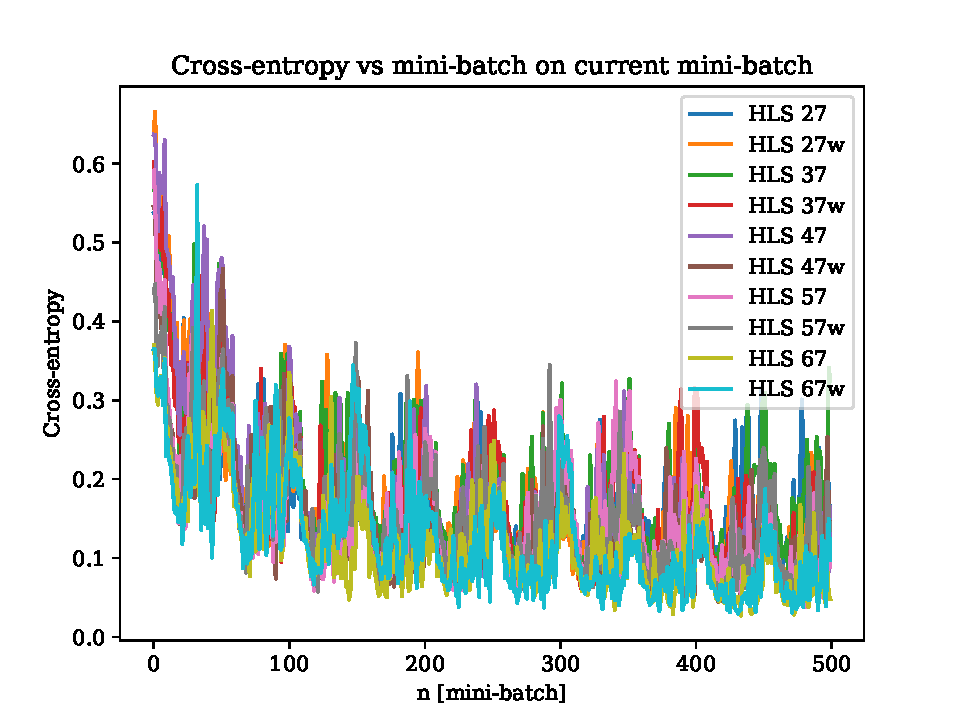
\includegraphics[width = \textwidth]{imgs/ps.pdf}
    \caption{Cross-entropy plot on the mini-batch for various initial sizes of the RNN, omitting first epoch. With and without the algorithm.}
    \label[fig]{E}
\end{figure}

\begin{figure}[h]
    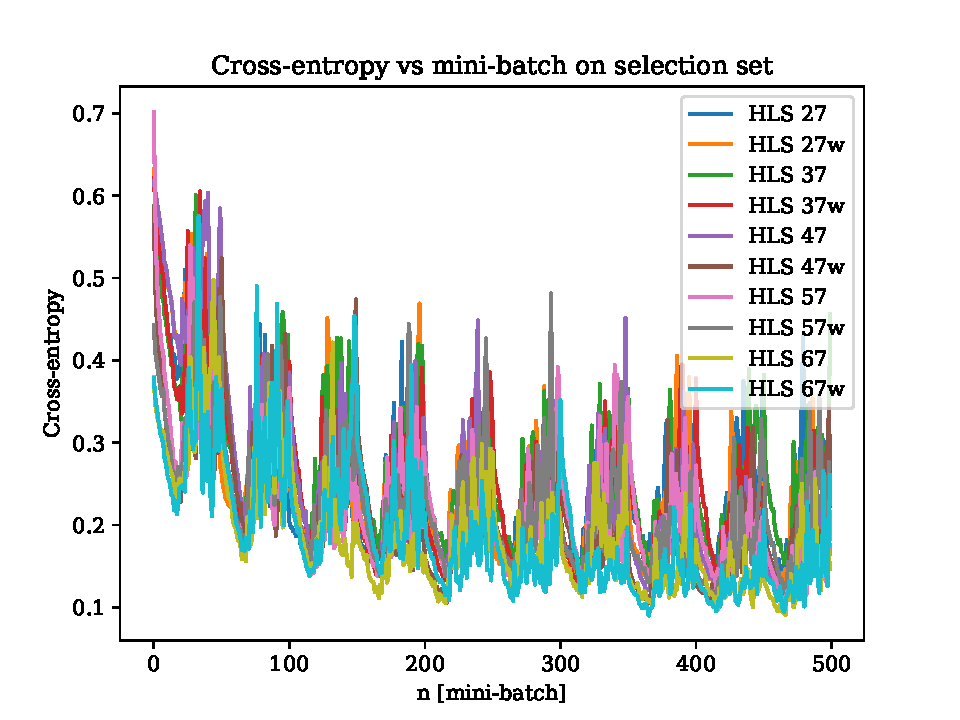
\includegraphics[width = \textwidth]{imgs/ps1.pdf}
    \caption{Cross-entropy plot on the selection set for various initial sizes of the RNN, omitting first epoch. With and without the algorithm.}
    \label[fig]{E_sel}
\end{figure}

As can be seen, a plot of energy during training. \ref{E} on the current mini-batch and \ref{E_sel} on the selection set. The variation is due to the mini-batch being a small subset.

\begin{figure}[h]
    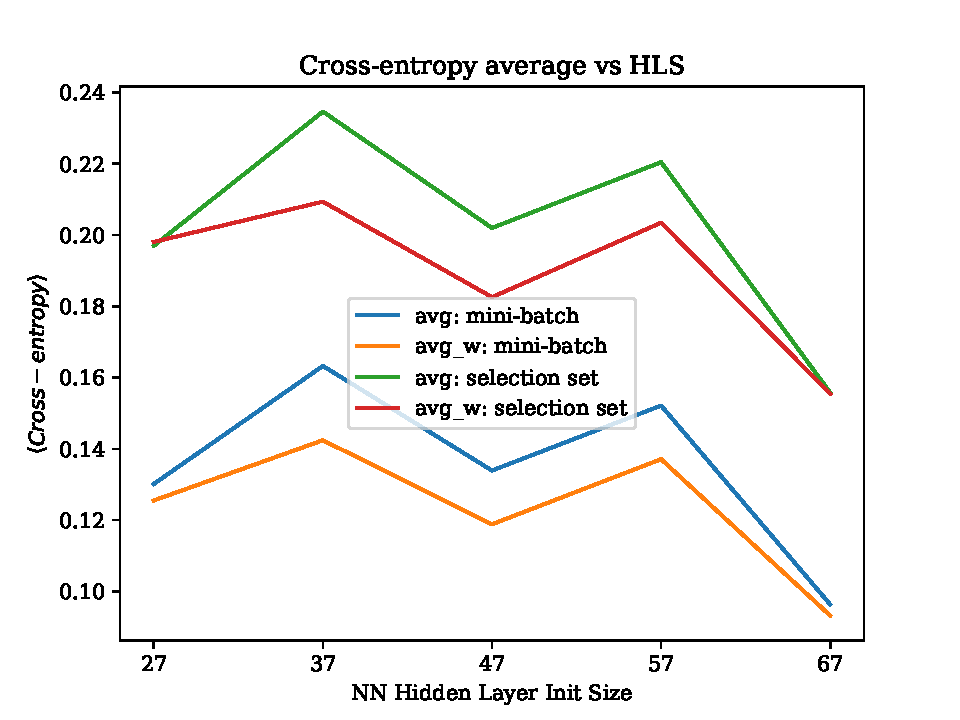
\includegraphics[width = \textwidth]{imgs/ps2.pdf}
    \caption{Average cross-entropy across training, after the first four epochs. For the mini-batch and sel, selection set. With and without the algorithm.}
    \label[fig]{avg}
\end{figure}

\begin{figure}[h]
    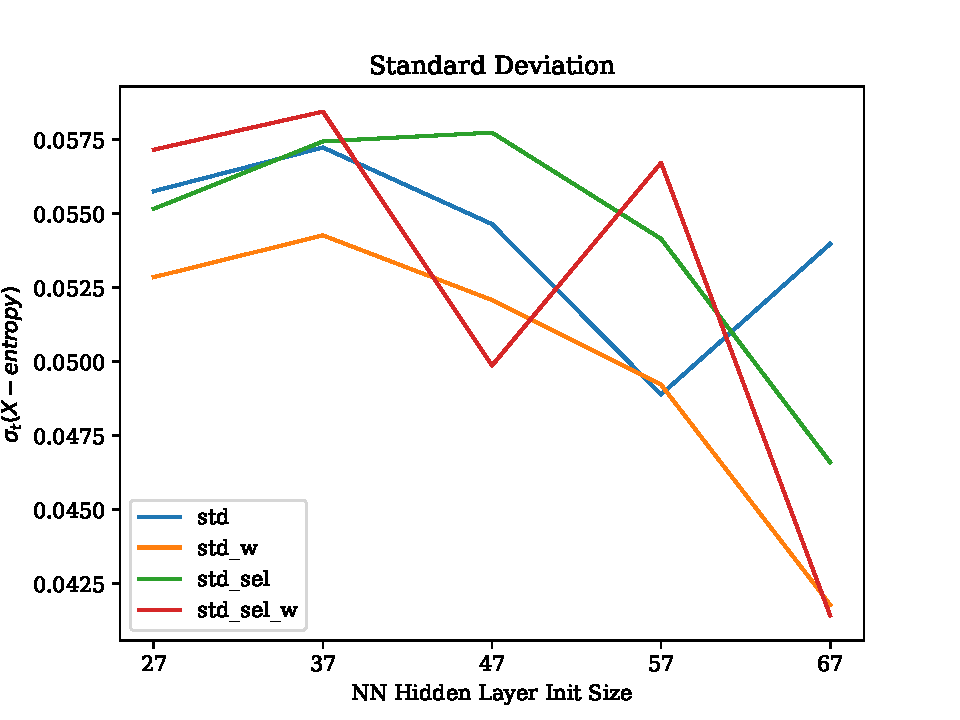
\includegraphics[width = \textwidth]{imgs/ps3.pdf}
    \caption{Standard deviation of the cross entropy across training, after the first four epochs. For the mini-batch and sel, selection set. With and without the algorithm.}
    \label[fig]{std}
\end{figure}

In the plots of the average \ref{avg} and standard deviation \ref{std}, a clear difference with or without the algorithm in the average which was stable. However, the standard deviation varied greatly depending on the number of epochs included in the calculation; this is due to randomly generated mini-batches.  

\begin{figure}[h]
    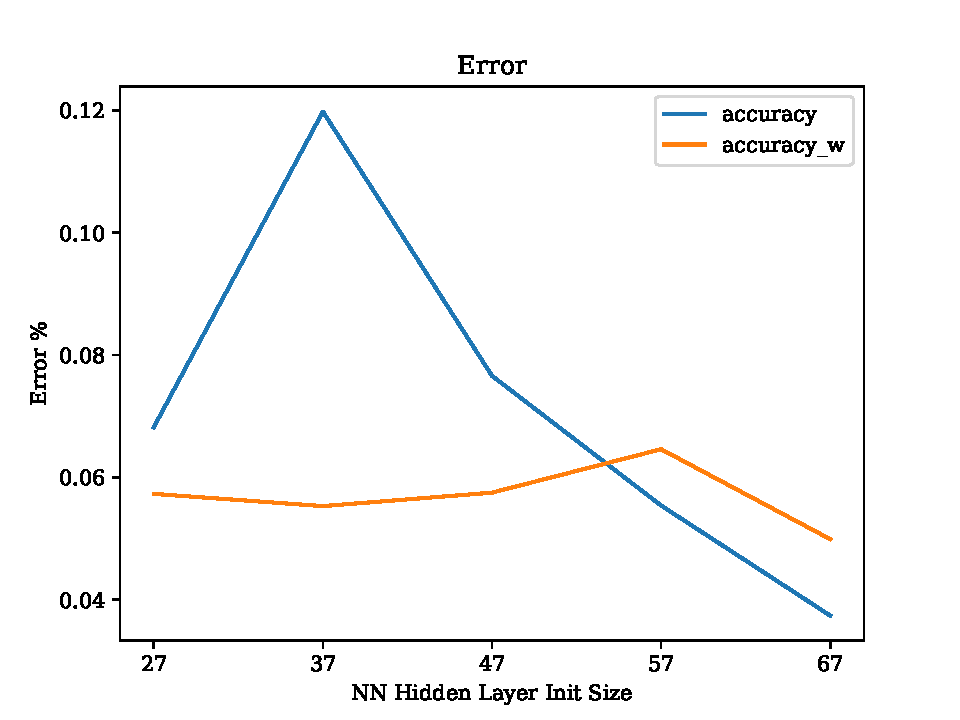
\includegraphics[width = \textwidth]{imgs/ps4.pdf}
    \caption{Error on test set, with and without the algorithm.}
    \label[fig]{acc}
\end{figure}

The last plot of the error on the test set \ref{acc} with and without the algorithm, which seems to perform well for small to medium-sized NNs.

\begin{table}[h]
    \centering
    \begin{tabular}{|l|l|l|l|l|l|}
    \hline
       Hidden Layer Size & 27 & 37 & 47 & 57 & 67 \\
    \hline
       - & 6.82 & 11.98 & 7.66 & 5.54 & 3.74 \\
    \hline
       w & 5.73 & 5.53 & 5.75 & 6.46 & 4.99 \\
    \hline
    \end{tabular}
    \caption{Error in \%, with and without the algorithm.}
    \label[table]{acc_t}
\end{table}

In the table \ref{acc_t}, the error can be seen in plain text, w for with the regularization.


    \chapter{Discussion}

As can be seen in the results, the algorithm performs well for small to medium sized NN. For the larger NNs, the increased size makes the induced changes relatively smaller, a remedy could be to perform multiple perturbations. For the really small NNs, the regularization was not so active as all moves or changes were rejected. This hints that, as expected, the really small NNs are slimmed and do not benefit from pruning or growing. 

As can be seen in the average and the error plot and table, the regularization seems to smooth the effects of the size of the NN. The $Es$ and selection plot are very rich in data and are hard to draw any conclusions from. 

To avoid the variation seen in the cross-entropy, bigger mini-batches could be used but this relates to the HF approach rather than the regularization. A way to combat the variation more akin to the regularization could be to employ algorithms employed in micro or canonical ensembles, rather than grand canonical ensemble.

The equal treatment of the different moves is not explored and neither is the activity of the algorithm. Simplifying and leaving out the relaxation could benefit these studies. 

    \chapter{Conclusions}

Monte Carlo Regularization is a method for reducing overfitting in neural network training. This thesis's purpose was the proof-of-concept of this regularization, which targets the network's nodes or connections and removes or duplicates them. In doing so, pathological redundance could be eliminated and beneficial inserted into the network. The effects of the method have been established, a significant improvement was found on the MNIST for small to medium-sized recurrent neural networks compared to recurrent neural networks of similar size without the method. Further study is required to establish a scaling in the activity of the regularization for larger NNs. The method is general and could be applied to arbitrary kind of neural network, the reason for using recurrent neural networks is that their non-linear structure complicate the benchmarking of structural perturbations.

The study and measurement of the hidden state size was omitted; however, a very rudimentary comment is that allowing for an increase in the hidden layer size directly increases the hidden state's size. Not included was the activity or selection of parameter of the method which should be properly studied. The neccesary scaling could be established accordingly. 

The regularization lengthened the training; however, comparatively, the Hessian-free optimization approach was the dominant part of the elapsed time. However, utilizing stochastic gradient descent could reduce the relative times, and optimizing the regularization could then be of importance. Speeding up the process overall, thereby not relying on a supercomputer, is a piece of advice for future study. Also, relying on existing libraries and open-source platforms for machine learning is a protip, not to reinvent the wheel in C++ but rather to depend on the flexibility of giants.

\section{Future work}

The algorithm hints at a method of initializing a network by continuously perturbing the network pre-training until some threshold value on a cross-validation set is met. 

A way to instead combat the standard deviation instability is regularizing the parameter update produced in the conjugate gradient method by perturbing and benchmarking it in a similar way to Monte Carlo Regularization on a selection set, inspired from micro-canonical sampling, which treats energy as a conserved quantity, to limit the effect on the selection set cross-entropy of a mini-batch update. The analogy is to a micro-canonical simulation. A demon considers changes in energy, for example, by producing an extensive update on the selection set and projecting smaller updates from mini-batches to update parameters by considering more information at each mini-batch or randomly benchmarking perturbing the generated updates.

Lastly, regulating the mini-batch size could be done similarly. If the selection set performance goes down to increase the mini-batch size and vice versa, somewhat like sampling different temperatures, regulating how much information is considered in each update of the NN parameters. Nevertheless, this relates to further study and merely is concepts derived from this successful regularization technique.

    \printbibliography

\end{document}